\subsubsection{Généralités}
\label{subsubsec:sonGeneralites}

L'arborescence des fichiers audios se matérialise comme suit:

\definecolor{folderbg}{RGB}{124,166,198}
\definecolor{folderborder}{RGB}{110,144,169}

\def\Size{4pt}
\tikzset{
        folder/.pic={
                        \filldraw[draw=folderborder,top color=folderbg!50,bottom color=folderbg]
                        (-1.05*\Size,0.2\Size+5pt) rectangle ++(.75*\Size,-0.2\Size-5pt);
                        \filldraw[draw=folderborder,top color=folderbg!50,bottom color=folderbg]
                        (-1.15*\Size,-\Size) rectangle (1.15*\Size,\Size);
                }
}

\label{fig:audioFilesTree}
\begin{forest}
        for tree={
        font=\ttfamily,
        grow'=0,
        child anchor=west,
        parent anchor=south,
        anchor=west,
        calign=first,
        inner xsep=7pt,
        edge path={
                        \noexpand\path [draw, \forestoption{edge}]
                        (!u.south west) +(7.5pt,0) |- (.child anchor) pic {folder} \forestoption{edge label};
                },
        % style for your file node 
        file/.style={edge path={\noexpand\path [draw, \forestoption{edge}] (!u.south
                                        west) +(7.5pt,0) |- (.child anchor) \forestoption{edge label};}, inner
                        xsep=2pt,font=\small\ttfamily }, before typesetting nodes={ if n=1 {insert
        before={[,phantom]}} {} }, fit=band, before computing xy={l=15pt}, }
        [src/ressources/audioFiles/USER [audio [UP [USER-UP1.wav, file] [..., file] ]
                [DOWN [..., file] ] [LEFT [..., file] ] [RIGHT [..., file] ] [OTHER [..., file]
                ] ] [model [..., file] ] [config.yaml, file ] ]
\end{forest}

\begin{figure}[H]
        \centering
        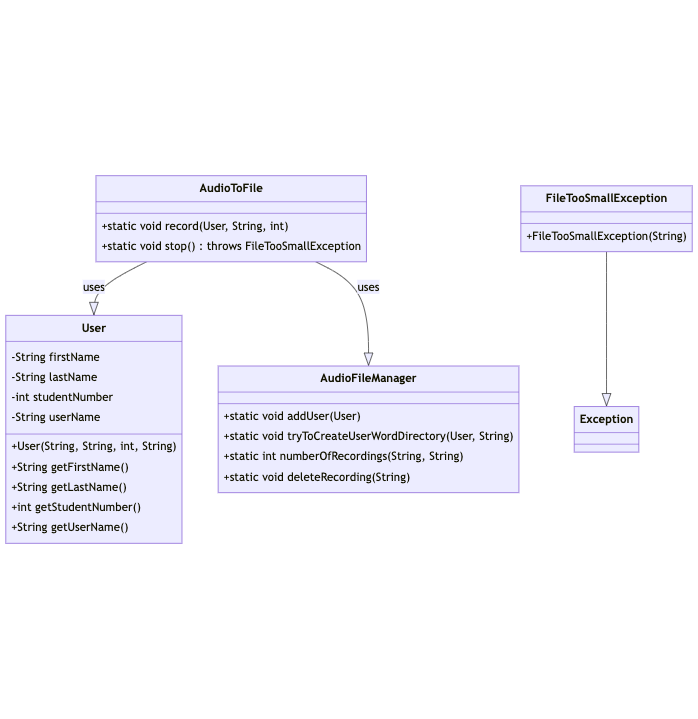
\includegraphics[width=10cm]{ressources/Implementation/Son/Audio.png}%
        \caption{Les classes liées aux fichiers audio}
        \label{fig:audioFilesClasses}
\end{figure}